\section{问题入口：CoT 为什么有效，也为什么显得笨重}
\label{sec:motivation-cot}

本章的结论先说清楚：思维链（Chain-of-Thought, CoT）的有效性来自外部化迭代。模型把中间步骤写成文本 token，随后把这些 token 放回上下文，借此获得多轮更新机会。它的沉重代价也来自同一个设计：每次内部状态更新都要经过“隐藏表示 \(\rightarrow\) 文本 token \(\rightarrow\) 隐藏表示”的窄门。Loop Transformer 的动机正是从这条窄门开始的。

\begin{importantbox}{本章主张}
推理能力需要可保存的中间状态和可重复执行的更新操作。CoT 用文本轨迹提供这两件事；循环 Transformer（Loop Transformer）试图把迭代过程放回模型内部的隐藏状态中。
\end{importantbox}

\subsection{测试时计算：推理模型为何愿意多花算力}

从第一性原理看，测试时计算（test-time compute）指推理阶段额外投入的计算量。一次普通前向传播像一次心算，模型必须在一次状态更新中给出答案；带 CoT 的推理像在纸上写草稿，模型可以先写出中间事实，再利用这些中间事实继续更新。

视频开头把主流推理模型、测试时计算、多跳推理、CoT、自一致性和自我修正放在同一张“推理能力冰山”图中。这个画面要表达的重点是：现代推理能力经常来自更长的推理过程，而更长过程通常意味着更多 token、更多采样路径，或者更多内部更新机会。

\begin{figure}[htbp]
    \centering
    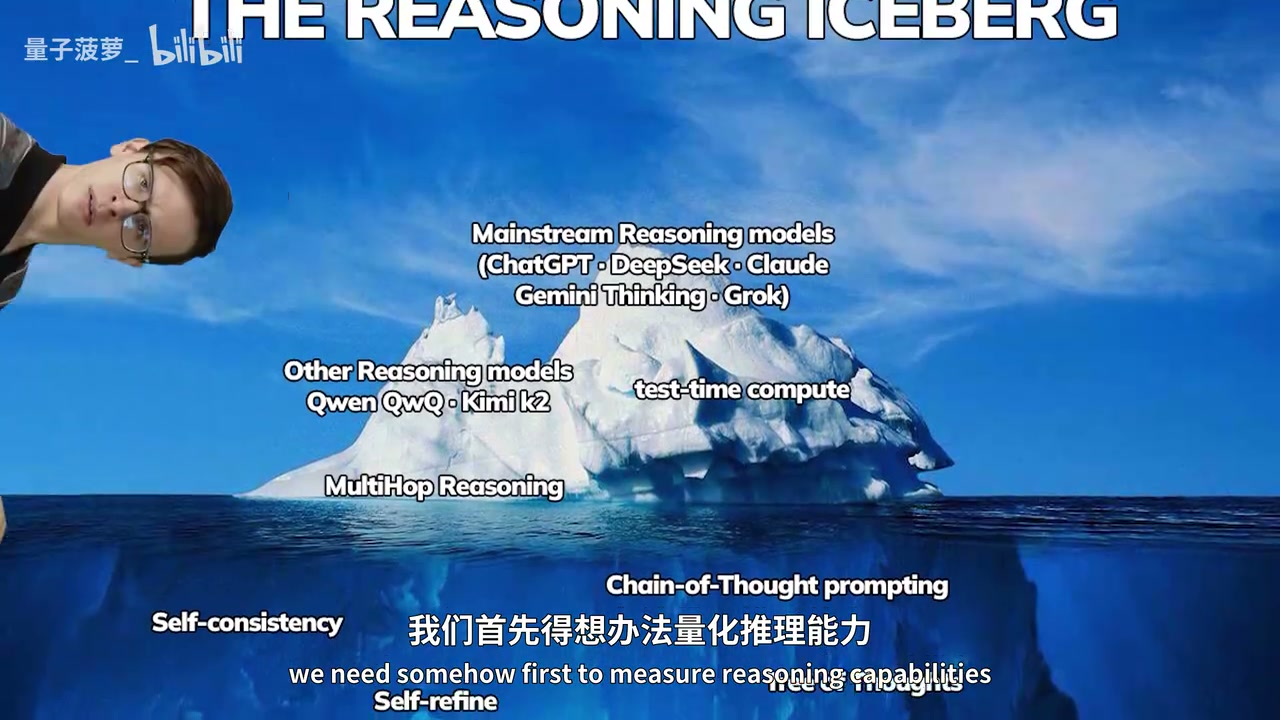
\includegraphics[width=0.82\linewidth,height=0.34\textheight,keepaspectratio]{figures/fig_01_reasoning_iceberg.jpg}
    \caption{推理能力冰山：多跳推理、测试时计算、CoT、自一致性和自我修正都在同一条“增加推理过程”的技术谱系上。\protect\footnotemark}
    \label{fig:reasoning-iceberg}
\end{figure}
\footnotetext{视频画面时间区间：00:02:29--00:02:39。}

更具体地说，测试时计算给模型提供三种机会。第一，模型可以尝试多条路径，减少一次采样失败带来的风险。第二，模型可以把复杂问题拆成较小的中间问题。第三，模型可以在后续步骤中修正前面步骤留下的粗糙表示。这里的关键词是“迭代”：没有迭代，复杂推理就会被压进一次前向计算中；有了迭代，模型至少获得了逐步改进的空间。

\subsection{多跳推理：从单步匹配到状态追踪}

多跳推理（multi-hop reasoning）是理解这件事的最小例子。视频给出的例子是：“谁是第 44 任美国总统的妻子？”这个问题需要两次跳转：先找到“第 44 任美国总统是 Barack Obama”，再找到“Barack Obama 的配偶是 Michelle Obama”。每一跳都会产生新的中间状态。

\begin{figure}[htbp]
    \centering
    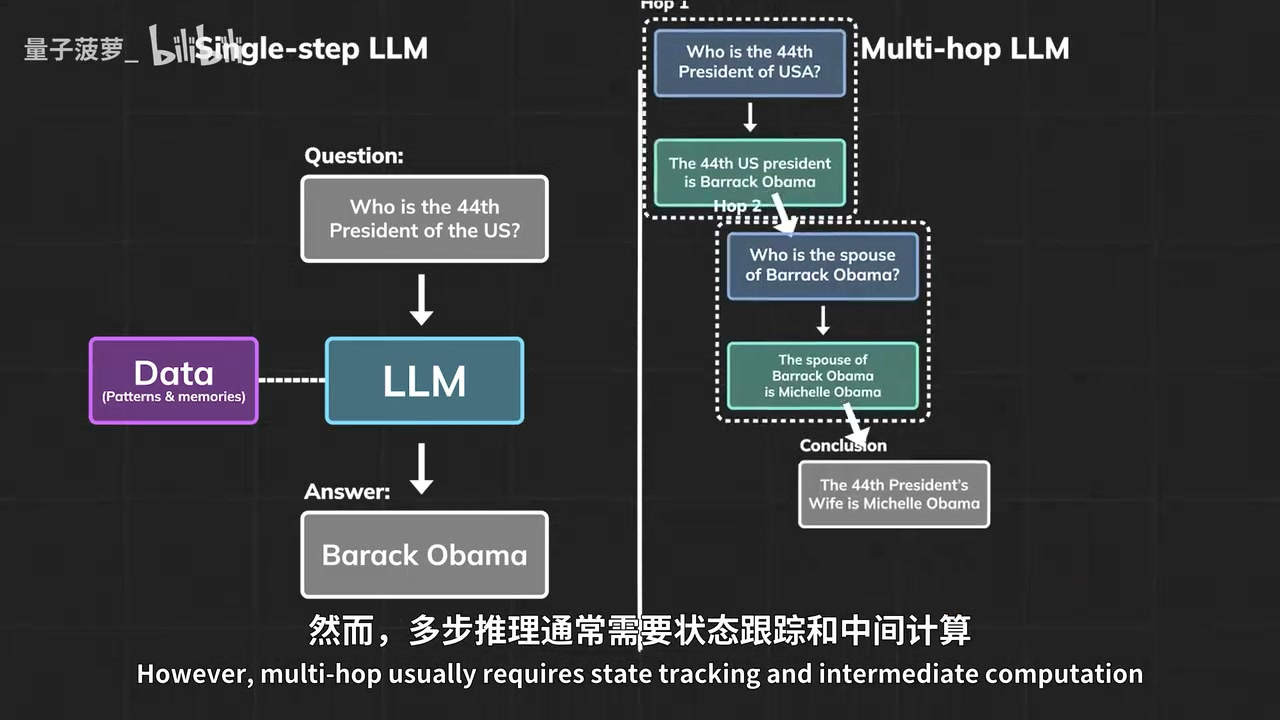
\includegraphics[width=0.82\linewidth,height=0.36\textheight,keepaspectratio]{figures/fig_02_single_vs_multihop_llm.jpg}
    \caption{单步问答更接近模式匹配；多跳推理要求模型维护中间状态，并把多个事实关系串成答案。\protect\footnotemark}
    \label{fig:single-vs-multihop}
\end{figure}
\footnotetext{视频画面时间区间：00:03:04--00:03:31。}

单步问答的难点通常是“有没有记住这个映射”。例如输入“第 44 任美国总统是谁”，输出“Barack Obama”可以近似看成从问题模式到答案模式的检索。多跳问题的难点更接近“能否保持工作记忆”。模型需要在第一跳之后保留中间答案，再把中间答案变成第二跳的查询条件。

\begin{knowledgebox}{把多跳推理想成查资料}
单步问题像在索引里查一个词条。多跳问题像先查一个词条，再把查到的结果当作第二个词条继续查。差别在于，中间结果必须被保存、引用和更新；一旦中间结果丢失，后续跳转就失去支点。
\end{knowledgebox}

这也是基础 Transformer 在多跳任务上容易吃亏的原因。若模型只能在一次生成中完成全部关系组合，它必须把所有中间计算压缩到当前隐藏表示中。跳数增加时，所需的内部计算深度也随之增加；缺少迭代机制的模型只能用参数记忆、注意力模式和一次性前向传播硬扛。

\subsection{CoT 的强处：用文本轨迹构造外部迭代}

CoT 改变了问题形态。模型先写出一个中间步骤，随后把这个中间步骤重新读回上下文，再生成下一步。这个过程让自回归模型获得了近似“循环”的效果：每一个生成的推理 token 都成为下一轮计算的输入条件。

按视频中的描述，CoT 的流程可以拆成四步：

\begin{itemize}
    \item 写出中间思考，例如先得到“第 44 任美国总统是 Barack Obama”。
    \item 回读已经写出的文本，把它并入当前上下文。
    \item 更新内部隐藏状态，让后续生成受中间结果约束。
    \item 继续写下一步，直到得到最终答案。
\end{itemize}

这解释了“多写 token 为什么能提高推理”。额外 token 承担外部状态存储的角色。文本轨迹让模型有地方放中间变量，也给训练者提供可观察的监督对象：可以筛选中间步骤，可以模仿高质量轨迹，也可以用强化学习偏好更好的推理路径。

\subsection{CoT 的代价：每次更新都穿过 token 窄门}

CoT 的笨重处也很直接：模型真正想优化的是隐藏状态中的潜在表示，实际执行时却要先把中间表示压成离散文本 token，再在下一轮把文本重新嵌入回隐藏状态。这个压缩、采样、追加上下文、再嵌入的环节让推理过程受 token 介质约束。

\begin{figure}[htbp]
    \centering
    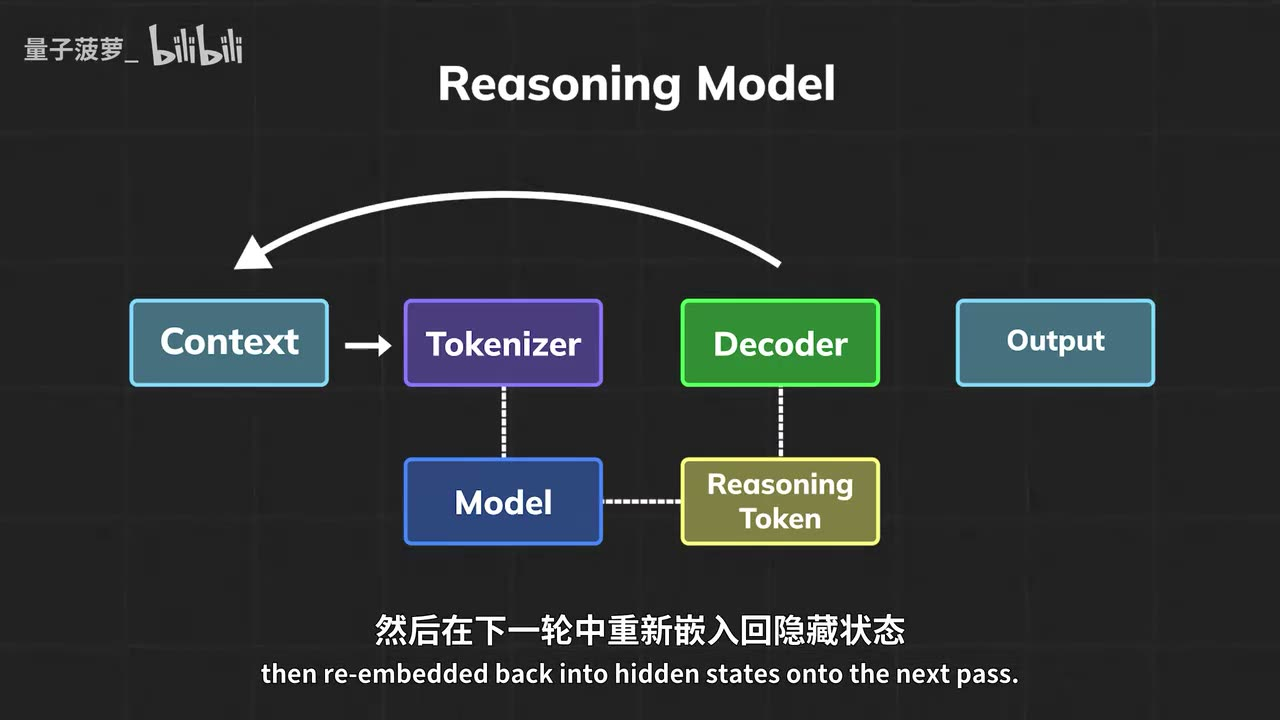
\includegraphics[width=0.82\linewidth,height=0.34\textheight,keepaspectratio]{figures/fig_03_cot_token_pipeline.jpg}
    \caption{CoT token 管线：模型把推理步骤写成 token，再把这些 token 追加到上下文并重新嵌入，形成外部化迭代。\protect\footnotemark}
    \label{fig:cot-token-pipeline}
\end{figure}
\footnotetext{视频画面时间区间：00:04:20--00:04:30。}

这张流程图给出了一条重要线索：CoT 的循环发生在文本上下文层面。模型生成 reasoning token 后，token 经过解码器形成文本输出，文本又被追加到上下文，随后重新进入 tokenizer 和模型。这个过程可以工作，甚至非常有效；代价是每一步推理都要支付离散化和上下文增长的成本。

\begin{warningbox}{常见误读}
“CoT 很重”并不等于“CoT 没价值”。它重在运行路径：中间状态要外化成 token，序列长度会增长，采样轨迹也会引入噪声。它有价值在监督路径：文本中间步骤天然可读、可筛选、可训练。后文讨论 Loop Transformer 时，这两条线需要同时记住。
\end{warningbox}

这就引出 Loop Transformer 的问题意识：如果推理的核心是反复更新隐藏状态，是否可以直接在隐藏状态中迭代？这个问题的意义超过“优雅”本身。它直接关系到计算路径、监督信号、缓存开销和部署成本。下一章会把这个直觉写成具体的循环更新机制。

\subsection{本章小结}

本章建立了后文的入口判断。第一，测试时计算提升推理的关键在于给模型更多路径和更多更新机会。第二，多跳推理把这种需求暴露得很清楚：模型必须维护中间状态，才能从一个事实跳到另一个事实。第三，CoT 通过文本 token 搭出外部迭代通道，因此有效；它同时把隐藏状态更新绑定到离散 token 管线，因此沉重。Loop Transformer 的核心动机就是把“写草稿再读回来”的外部循环，改写成隐藏状态上的内部递归。
